\chapter{ODD Documentation of the Agent-Based Model} \label{appendix-odd}

The core model is documented below using the `overview, design concepts, and details' (ODD) standard \cite{grimmODDProtocolReview2010a}. Following Grimm et al. \cite{grimmODDProtocolDescribing2020} this ODD consists of seven elements (Figure 1):

\begin{enumerate}
    \item Purpose
    \item State variables and scales
    \item Process overview and scheduling 
    \item Design concepts
    \item Initialization
    \item Input and 
    \item Submodels 
\end{enumerate}
% Conceptually the elements fall into the three categories ``Overview,'' (1-3) ``Design concepts'' (4, with subcategories)  and ``Details''; hence the acronym ODD.

Chapter~\ref{chapter-methodology}, on methodology, gives more detail on the modelling purpose, strategy, and type, The formulae used in the model are described and explained in Chapter~\ref{chapter-model}, the model chapter. Appendix~\ref{appendix-parameters} provides parameter values.  The exposition in this chapter is strictly descriptive and what the model includes and does.

\section{Purpose}
% TODO add in purposes of modelling work - The purpose of this model is to understand ..Following xyz, xyz gives x purposes for modelling.
The purpose of this model \gls{theoretical exposition}. More specifically, we seek is to understand the links between financialization and  the distribution of housing ownership, the capture of rents, and  urban productivity. %, through financialization of the urban housing market. 
Our  qualitative positive results on these issues provide valuable directions for further quantitative research.

\section{State variables and scales}
\subsection{State variables}
State variables refer to the attributes of each kind of entity that vary over time.%\footnote{In the ODD framework, state variables commonly refers to both stock variables and parameters. Although it is inconsistent with usage in the analysis of dynamical systems, we follow the ODD convention in this section.}. 
The entities in our model are persons, land units (properties or lots), a representative urban firm, an investor, a bank, and a realtor.
\footnote{The agents are described in the agent section of the code.} The city is the entity or model that includes the agents. The city administration is not an agent. %  who may choose to work at an urban firm, properties, each occupying a an urban grid space. %, 

State variables for the system are: number of workers (population),  worker savings, number of firms, workers per firm, capital stock per firm, city area, housing stock owned by workers, housing stock owned by investors, and wage level.

\subsubsection{Persons}
Rural and urban owner-occupiers and tenants belong to the class Person. Newcomers are the subset of rural persons entering the urban workforce in a period. They become owners or tenants. Urban owner-occupiers and tenants make up the primary workforce. %(The city has a small and fixed core population.) 

The state variable (attributes) for persons are property location, initial working period (providing age), savings, ownership status, capital gains tax level, ownership status, and property owned. Mortgages payments or rental payments are calculated to update savings. Each person occupies one property. 

Persons can choose to work or not work in the city, depending on wages and transportation costs. If the wage justifies travel to the city center, persons with properties at the edge of the city join the urban workforce as owner-occupiers. 

Persons have a 40 period working life, after which they retire and list their home.  
Retirees are replaced by newcomers from the rural region who bid on properties. Tenants do not bid but may be replaced by newcomers who do bid. If newcomers make a successful bid they become owner-occupiers. If they fail, they become tenants. If investors outbid tenants and newcomers, they become non-resident owners.  

\subsubsection{Properties}
Properties belong to the class Land. The state variable  for properties are location, transport cost, property tax rate, maintenance costs, warranted price, warranted rent, appraised price, realized price, price change, ownership type, owner  
%not occupancy status ?

\subsubsection{Bank}
The bank is the sole member of the class Bank. It sets maximum mortgage share and credit-worthiness using person attributes and bank parameters. It sets lending rates for persons and investors based on the prime rate. Mortgages payments are calculated for a 5-period term.
 
\subsubsection{Investors}
A representative  investor is the sole member of the class Investors.   A fraction of investor owned properties are listed  for sale in each period.

The state variables  for the investor are borrowing interest rate, the A fraction of investor owned properties are listed  for sale in each period, properties owned, a capital gains tax rate, expectations about the rate of price change,

\subsubsection{Realtor}
The realtor keeps lists of properties for sale and for rent in each period, conducts bidding, and allocates properties to the winning bidder.

The realtor interacts in each period with listed properties and  all bidders, but has no state variables.


\subsubsection{Firm}
A representative firm is the sole member of the class Firm. It has a production function, a workforce, capital stock and a wage 

The firm is a complex entity. The state variables for the firm are output price and wage (consisting of subsistence wage plus an urban wage premium), a production function with parameters  A, alpha, beta, and gamma. A is dependent on interaction with the ownership ratio. The agglomeration population for the production function is calculated in the firm using the urban seed population, density and a multiplier. The cost of labour considered in hiring includes overhead. The overhead parameter can be used to explore the effect of payroll taxation.

Firm-determined variables evolve from current values toward target values according to partial adjustment rules. The adjustment rates are specified in the code.  

                
\subsection{Scales}

The computational field is a grid of properties, typically set to 130 properties by 130 properties, which is sufficient to contain the city and still leaving properties in the `rural' state in every direction after a typical .
100 period run. One hundred model cycles are intended to represent 100 chronological years of city development. Longer or shorter runs are often convenient. 

Each property has one resident. (This is a computational convenience that exploits our decision to have a single person type and a uniform density. At the cost of additional computation properties can have different densities and diverse person-types.) 

The city has a density parameter which multiplies the the number of properties by a density number to get the basic city population. 

The population determines the magnitude of the agglomeration effect that enters the firm's production function.

Not all the parts of our model are at the same level of resolution. We combine coarse generalizations about long-term agglomeration effects with fine-grained housing and financial market processes. our goal is to examine in moderate detail how financial decisions affect home ownership while black-boxing the transmission of agglomeration effects through firms from aggregate productivity gains to population growth. 

% There are x types of agents. They have the state variables outlined in the tables. 

% variables can include behavioral attributes and model parameters.
% Variables include the model’s entities, their state variables (possibly including behavioral attributes and model parameters), and the model’s spatial and temporal scales.

% Environment variables include XXX

% Overview of process, parameters and default values for the xx model

\section{Process overview and scheduling}

The model proceeds in discrete steps. Each time step represents one year.  Agents use state variables from the prior time step. Agents of a particular kind execute their step function in randomized order.  Figure~\ref{fig:computational-sequence} illustrates the sequence in which function are called. Figure~\ref{fig:information-flows} illustrates the major information flows between agents and functions.

\begin{figure}
\centering \vspace{-2cm}
\begin{tikzpicture}[node distance=1.5cm]
\node (init) [startstop] {Initialization};
\node (interventions) [process, below of=init] {Model applies interventions};
% \node (record) [process, below of=interventions] {Record ownership share and reset counters};
\node (mainloop) [startstop, below of=interventions] {Main loop};
\node (firmupdate) [process, below of=mainloop] {Firms update wages based on number of workers};
\node (land) [process, below of=firmupdate] {Land records data and computes price forecast};
\node (actions) [process, below of=land] {People choose to work based on wages, retire, and list properties};
\node (investors) [process, below of=actions] {Investors list properties};
\node (newcomers) [process, below of=investors] {Newcomers bid on properties};
\node (bid) [process, below of=newcomers] {Investors bid on properties};
\node (realtors_sell) [process, below of=bid] {Realtors sell homes};
\node (realtors_rent) [process, below of=realtors_sell] {Realtors rent properties};
% \node (store) [process, below of=realtors_rent] {Model stores data};
\node (advance) [process, below of=realtors_rent] {Model stores data and advances time step};

\draw [arrow] (init) -- (interventions);
% \draw [arrow] (interventions) -- (record);
% \draw [arrow] (record) -- (mainloop);
\draw [arrow] (interventions) -- (mainloop);
\draw [arrow] (mainloop) -- (firmupdate);
\draw [arrow] (firmupdate) -- (land);
\draw [arrow] (land) -- (actions);
\draw [arrow] (actions) -- (investors);
\draw [arrow] (investors) -- (newcomers);
\draw [arrow] (newcomers) -- (bid);
\draw [arrow] (bid) -- (realtors_sell);
\draw [arrow] (realtors_sell) -- (realtors_rent);
\draw [arrow] (realtors_rent) -- (advance);
% \draw [arrow] (store) -- (advance);

\draw [arrow] (advance.south) -- ++(0,-.5) -- ++(7,0) |- (mainloop);
% % Custom arrow path
% \draw [arrow] ($(advance.south) + (0,-0.5)$) -- ++(0,-1) -- ($(mainloop.south) + (-2,-1)$) -- ($(mainloop.south) + (-2,0)$) -- (mainloop);

\end{tikzpicture}
\caption{Computational sequence} \label{fig:computational-sequence}
\end{figure}


Persons initially have locations. They choose whether to work or not work, based on the wage premium and transportation costs, thus determining if their location is in the commuter-shed. This step determines the extent of the city and its population. Persons remain in the workforce until they reach retirement age. If people are above the retirement age, they retire and list any properties for sale if they are moving out of the city. 


 % The sequence of the code means agents do not use information from, or interact with agents of the same type during their step function, so the order doesn't matter.

In each time step, the representative firm computes the value of the marginal worker's value product at current prices, chooses a new target workforce and a new target wage. It follows a partial adjustment rule in choosing wage, labour force, capital stock for the following period. Firm size is constrained by diminishing returns to scale. New firms enter when population grow beyond what existing firms target. 


The the wage premium is calculated from the wage  and used by agents to decide whether to work in the city,.

Each unit of land (lot) is an `agent.' Each uses the wage premium and its own location (plus any other attributes) to compute its locational value (warranted price) and potential rental earnings. 

The Bank function determines mortgage availability for newcomers and tenants. 

Newcomers and investors bid on properties listed for the period. They use an expected price includes information about how the market has behaved, so it is possible for price bubbles and expectations to feed back into the dynamics. 

A Realtor function takes the list of bids and mimics a bargaining process to reach a final price. if possible. If the owners will not occupy their own houses, properties are rented to newcomers who are included in the tenant count.



% Overview of process, parameters and default values for the xx model
% - description of the model’s schedule that is detailed and precise enough to allow the model to be re-implemented.
% - schedule descriptions based on pseudo-code most useful.


\section{Design concepts}

% Basic principles
% Adaptation - adaptive traits - rules for  how changing in response to changes in environment or themselves. do they seek to increase some measure
% Objectives - what is the objective and how is it measured
% No - Learning - change adaptive traits based on experience
% Prediction - the anticipate based on past prices


We combine two distinct approaches to modelling social systems: agent-based and equilibrium modelling.  We use equilibrium conditions for competitive labour markets to bypass the complex and partially understood wage-setting process. We also use equilibrium arguments to compute land rents from the transportation cost and urban wage premium that drive urban locational decisions. Chapter~\ref{chapter-methodology}, on methodology details the decisions about model type. The equilibrium models provide the environment for  our   agent-based migration and  housing market models.

For simplicity, we present the model for the case where individuals have the same preferences, employment opportunities and transportation costs. The principles explored include the relationship between urban agglomeration effects and the financialization of the urban housing market. The model also expresses several other concepts as described below.

\subsection{Emergence}
% The class structure is emergent in our model, in that it's not in the base sent of specified objects, but it is a structure that appears through the interaction of agents in the model rather than one specified initiallty.

% PI "today's theoretical physics is tomorrow's technology"

% Roemer defines class as 
% class relations are determined by individuals' ownership or non-ownership of productive assets, such as labour,  machinery, factories, or, in our case, land. Exploitation occurs when someone gets their income from the productivity of someone else's person or assets. 

% In this sense, 
There are four social classes in our model: urban owner-occupiers  urban tenants, rural owner occupiers and investors. The city itself and the urban owner-occupier is an emergent entity that bubbles up out of the rural economy as a result of agglomeration economies. We begin our exploration after the city emerges. In the regime we study, the tenant and investor classes are also emergent. Introducing additional differences among agents would open the possibility of urban segregation and the endogenous emergence of further \gls{class} distinction based on  access to various forms of capital, a process explored by John Roemer in his General Theory of Exploitation and Class \cite{roemerGeneralTheoryExploitation1982}.
% Ownership, the regime, emerges, advantage are amplified leading to a different end state.They correspond to social classes  

There are two possible pure urban regimes, An owner-occupier regime and a tenant regime which investors own all properties. We start our experiments with a pure owner occupier regime in which those who own houses and work can build equity.  The city may then transitions toward the investor-owned regime as investor-agents purchase properties based on local expected financial return calculations. Our experiments explore some policy interventions that could affect the transition.

%We model individual agents' access to finance, %and the cost of money we introduce an innovation to formal urban modelling. We 
%drawing on the literature for the relevant `\gls{stylized facts}' about differences in individual financial access based on wealth and income. 

\subsection{Adaptation, learning and prediction}
There is no learning in the sense that agents do not change their traits based on experience. 
Agents do make predictions, anticipating prices based on the rate at which those prices have increased in the past $\dot P$.

\subsection{Sensing}
All agents have information about the wage, warranted price, expected and their own borrowing costs. They make their decisions based on what is best for them. 

\subsection{Interaction}
Agents get information from the firm about wages. They independently make decisions to work or retire, but because of agglomeration effects, their decision to work and it's effect on the size of the labour market feed back to affect wages in the next step. 

The central interaction  is in the housing market through the competitive bidding process that allocates properties and rents.  A secondary interaction occurs if the allocation of housing or rents influences the production function as described in chapter~\ref{chapter-tramsmission}.

\subsection{Stochasticity}
Stochasticity comes into the main model two ways: through the range of initial agents and savings, and through randomising the order in which which agents act. When multiple runs re made with the same parameter settings these stochastic elements only produce variation in the evolution of the ownership ratio unless the ownership ratio affects productivity. With linkages all the outcome variables will vary slightly.

% For testing the model's sensitivity to parameters, we use a version that shortcuts the land market and bidding process by directly calculating equilibrium population.  This version lacks the stochastic elements built into the land market sub-model. It is much faster computationally.

\subsection{Feedback loops}
Feedback loops are not part of the ODD standard, but an important concept in this work. 
% https://en.wikipedia.org/wiki/James_J._Kay
% https://www.researchgate.net/scientific-contributions/James-J-Kay-2162967174
% https://uwaterloo.ca/systems-design-engineering/about-systems-design-engineering/department-history
There are three \glspl{feedback loop} in the model: the productivity-wage, population-productivity loop that we call the Alonso-Jacobs cycle,  the speculative investment-price, inflation-investment cycle that may produce price bubbles, and the feedback from ownership to the production function, which then affects population, wages an ownership.\footnote{Feedback loops are a fundamental feature of almost all systems. They have probably been recognized by theorists for centuries. Marx, to take one relatively modern example, identified the growth dynamic of the capitalist system  as a feedback loop, with capital investments producing a surplus that was fed back into investment, growing the stock of capital. Marx claimed that this loop produced dynamic instability and a great deal of subsequent work has supported his insight \cite{dumenilStabilityInstabilityDynamic1986} \cite{schumpeterInstabilityCapitalism1928}. More recently, the Keynesian multiplier is a result of feedback in macro models between expenditure and jobs. That loop produces a stable equilibrium. Neoclassical growth theory built on that mechanism to explore the determinants of economic growth using differential and difference equations. % Forrester, the creator of system dynamics computer simulation modeling, argued that change over time is caused by the process of accumulation CITE.
% The feedback concept formally entered the social sciences through two channels: cybernetics, pioneered by Nobert Wiener  and the participants of the Macy Foundation Conferences, and the servomechanism/control engineering thread championed by Jay W. Forrester and others. Both threads were picked up and applied by prominent economists.\footnote{Richardson \cite{richardsonFeedbackThoughtSocial1991} mentions Oscar Lange (1970), Kenneth Boulding, and Alfred Eichner, Phillips,  R. G. D. Allen (1956), and Axel Leijonhufvud.} There is now a niche sub-discipline in economics called ``Feedback Economics'' \cite{radzickiIntroductionFeedbackEconomics, cavanaFeedbackEconomicsEconomic2021}. %  and a great deal of work in The servomechanism/control engineering thread is the one most closely related to \gls{system dynamics} modeling and to ideas used in this thesis.
}
 
% Our model incorporates two important feedback loops. One, driven by agglomeration, we call the \Gls{Alonzo-Jacobs cycle}. The other is a price-financialization feedback that directly changes the ownership pattern in the urban housing market. 
The loops are linked. Rising productivity raises wages which then works through two paths. It can raise rents, effectively transferring productivity gains to landowners, and it draws more workers into the city workforce, enhancing the \Gls{Alonzo-Jacobs cycle}. 

%A rapid increase in housing prices may choke off urban population growth and cause the \Gls{Alonzo-Jacobs cycle} to stall. Rapid expansion of the housing stock should have the opposite effect. 
Much depends on the speed of response of the city population and the rate of transmission of agglomeration effects to wages through the firm. Our base model allows the boundary to respond to increments the wage with a small lag. In the base model, financial flows are unrestricted but the rate of financialization is limited by the rate of turnover of ownership. We parameterize the rate of adjustment for each of the stocks in a simple way in order to conduct sensitivity analysis.

\subsection{Observation}
The model records a large number of computed variables for diagnostic purposes, but output the variables we report are  the urban wage, land prices, city size, owner-occupier population, tenant population and total urban population, who owns which property, previous prices, firm capital stock, firm workforce size, and number of firms.

\section{Initialization}
Initial values for the model are detailed in Appendix~\ref{appendix-parameters} on initial values.

\section{Input}
The model does not draw on any digital datasets. Parameters have been chosen to be in j=ranges consistent with  theory and, where possible, empirical work. The combination of parameter values for the production model were chosen to produce a plausible growth trajectory for a city that grows from a small to large over a reasonable time period. To explore the model dynamics interventions, we can change key parameters mid-run to represent shocks to the system, to model labour market and price shocks and cyclical patterns. We do discuss the settings or the calibration process because the production model is simply the environment for  our agent-based exploration of the housing market.  % time varrying data. 

\section{Submodels}
There are three submodels: the spatial structure of the model, with each land unit having a transportation cost based on its distance from the urban center; the firm model that produces the urban wage; and finally the land market model that allows homeowners and financialized investors to bid on properties in order to capture the rising rents due to agglomeration.  


% \section{DIAGRAMS AND FLOW}

% Initialization
% Apply interventions
% Record ownership share and reset counters

% Main loop
% Firms update wages based on how many people choose to work in the city
% Land records locational rents and calculates price forecast
% People decide whether to work, retire, and list properties to sell
% Investors list properties to sell
% Create newcomers to purchase properties for sale
% Investors bid on properties
% Realtors sell homes
% Realtors rent properties
% Store data
% Advance model

\begin{figure}
\centering\vspace{-3cm}
\begin{tikzpicture}[scale=.3,node distance=1.5cm]
\node (init) [startstop] {Initialization};
\node (interventions) [process, below of=init] {Model applies interventions};
% \node (record) [process, below of=interventions] {Record ownership share and reset counters};
\node (mainloop) [startstop, below of=interventions] {Main loop};
\node (firmupdate) [process, below=1cm of mainloop, text width=5cm] {Firms update wages, number of workers, capital  based on prior wage};

\node (rural-boundary) [process, right=.5cm of firmupdate, text width=5cm] {boundary-adjacent owners decide to join or leave workforce};
\node (rural-remote) [process, below=.5cm of boundary-owners, text width=5cm] {Remote rural agents decide to join or leave workforce};


    \node (Remote-bid) [process, below=2.5cm of firmupdate, text width=5cm] {Remote rural agents bid for housing};
    \node (Invest-bid) [process, below=2.5cm of firmupdate, text width=5cm] {Investors bid for housing};
     \node (invest-list) [process, below=2.5cm of firmupdate, text width=5cm] {Land records data and computes price forecast};

\node (retired-list) [process,  left=1cm of land, text width=5cm] {Owners choose to  retire, list properties};
         \node (investors) [process, right=1cm of land] {Investors list properties};

        \node (realtors_sell) [process, below = .5cm of bank] {Realtors sell homes};
        \node (bank) [process, below = .5cm of land, text width=5cm] {Bank calculates mortgage availability};

\node (Owner-adjust) [process, below=2cm of actions, left=2cm of realtors_sell, text width=4cm] {Newcomers bid on properties};
\node (tenant-adjust) [process, below=2cm of actions, left=2cm of realtors_sell, text width=4cm] {Newcomers bid on properties};
\node (Agglom-adjust) [process, right=2cm of realtors_sell, text width=4cm] {Investors bid on properties};

\node (realtors_rent) [process, below of=realtors_sell] {Realtors rent properties};
\node (store) [process, below of=realtors_rent] {Model stores data};
\node (advance) [process, below of=store] {Model stores data and advances time step};

\draw [arrow] (init) -- (interventions);
% \draw [arrow] (interventions) -- (record);
% \draw [arrow] (record) -- (mainloop);
\draw [arrow] (interventions) -- (mainloop);
\draw [arrow] (mainloop) -- (firmupdate);
\draw [arrow] (firmupdate) -- (actions);
\draw [arrow] (firmupdate) -- (land);
\draw [arrow]  (actions) -- (land);
\draw [arrow]  (investors) -- (land);

\draw [arrow] (land) -- (bank);
\draw [arrow] (bid) -- (realtors_sell);
\draw [arrow] (newcomers) -- (realtors_sell);
 \draw [arrow] (bank) -- (newcomers);
% \draw [arrow] (investors) -- (newcomers);
% \draw [arrow] (newcomers) -- (bid);
% \draw [arrow] (bid) -- (realtors_sell);
 \draw [arrow] (realtors_sell) -- (realtors_rent);
 \draw [arrow] (realtors_rent) -- (store);
\draw [arrow] (store) -- (advance);

\draw [arrow] (advance.south) -- ++(0,-.5) -- ++(30,0) |- (mainloop);
% % Custom arrow path
% \draw [arrow] ($(advance.south) + (0,-0.5)$) -- ++(0,-1) -- ($(mainloop.south) + (-2,-1)$) -- ($(mainloop.south) + (-2,0)$) -- (mainloop);

\end{tikzpicture}
\caption{Information flows}
\label{fig:information-flows}
\end{figure}

\begin{figure}

    \centering
    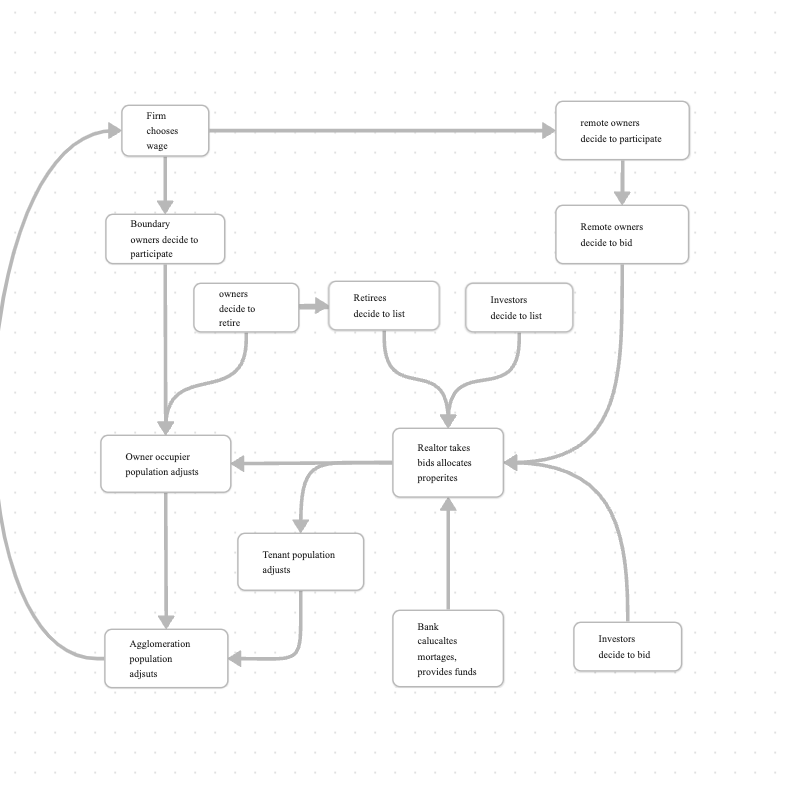
\includegraphics[width=1\linewidth]{informationflows.png}
    \caption{Enter Caption}
    \label{fig:information-flows}
\end{figure}

\subsection{Expectations}
\Glspl{expectation} matter in models of human systems because they introduce a mental model of the future state of agents in the model into current decisions.  We employ a simple backwards-looking expectation formation anchored 
%  This ANCHORING IS INTERESTING, BY THE WAY
to current rental returns.\footnote{Forecasts based on recent price movements can give rise to \glspl{price bubble} through either speculative or precautionary motives. Expectations anchored in \gls{perfect foresight} have different dynamics since agents correctly forecast the path of prices \cite{muthRationalExpectationsTheory1961}.  We describe an investment rule of this sort in Chapter~\ref{chapter-financialization} on financialization.} 
%Combining a spatially explicit agent-based model of the housing market with equilibrium models of rent and urban production allows us to stay close to the analytic tradition, and connect the work with both classical and neo-classical theory. 
% As pointed out above, we rely on equilibrium arguments in our model to ``black box'' the production sector and most of the labour market, including most decisions by producers and wage demands by workers.  


% \subsubsection{SORT - single value frontier - explore reasons}
% WHERE TO EXPAND% *** We will explain why the rent charged to the tenant is locked  to a single value. A few factors - we are looking at the frontiers- the economically justified maximum as a way of linking productivity and extraction formally. - there are many variations and extensions to build on/explore/relax these core assumptions - - want to do this for a few reasons \dots



%  It follows that 
% \[\frac{\partial U_i(d, d(dots)}{\partial t}=\frac{\partial U_j(d, /dots)}{\partial t}\]
% Finally, our model of the financial sector falls between the two approaches: each property transaction decision is made individually as it would be in an agent-based model, but we don't track individual investors. Our investor is technically an agent in the agent-based modelling sense, but the agent is the entire class of financial investors in housing, which is to say, a representative agent. Interestingly, perhaps, each property is also formally an agent with a set of attributes such as location, density, and ownership status. 





% \subsection{Marginal vs inframarginal quantities}
% In relying on these equilibrium conditions, we are implicitly applying standard neoclassical economic methods although our focus is not on the \gls{marginal} conditions that determine prices, but on the \gls{inframarginal} quantities that make up rents. We can illustrate with a diagram that illustrates the disnction between marginal and inframarginal (explained in more detail in Chapters~\ref{chapter-rent} and \ref{chapter-space} on rent and space respectively). 

\vspace{.3cm}
\begin{figure}[h!t!]
\centering
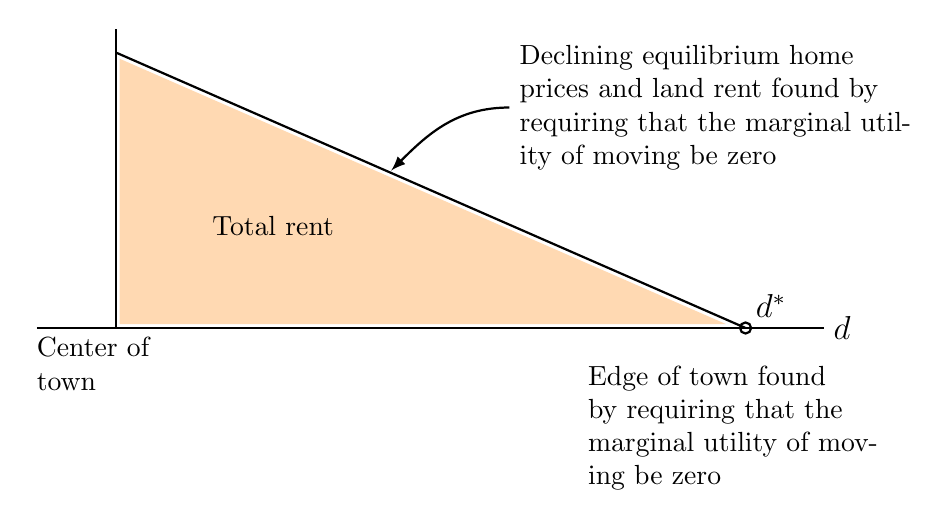
\begin{tikzpicture}[domain=0:2]
%\draw[thick,color=gray,step=.5cm, dashed] (-0.5,-.5) grid (3,3);
\draw[line width=.01] (0,0) -- (10,0) node[right] {\large $d$};
\node at (1,0) [below,text width=2cm] {Center of town};
%\draw[thick ] (0,3)node[above right] {merchant's price in town} -- (10,3) ;
\draw[thick ] (0,0)  -- (10,0); 
\draw[thick, -latex] (6,2.8)
node[right, text width=5cm]{Declining equilibrium  home prices and land rent found by requiring that the marginal utility of moving be zero} 
to [out=180, in=45](4.5,2); 

\fill[orange!30] (1.05,0.05)--(8.75,0.05)--(1.05,3.42)--cycle;

\draw[thick ] (1,0) -- (1,3.8);
\draw[thick ] (9,0)node [above right]{\large $d^*$}circle[radius=2pt] node[below=.35cm,text width=4cm] {Edge of town found by requiring that the marginal utility of moving be zero} -- (1,3.5) ;

\node at (3,1.3){Total rent};
\end{tikzpicture} 
\caption{Illustrating marginal and infra-marginal quantities with the bid-rent curve and aggregate rent.}
\label{fig-land-rent-as-inframarginal}
\end{figure}

In Figure~\ref{fig-land-rent-as-inframarginal}, The level of rent is determined at any distance by individuals making comparisons locally. At point $d^*$ the person at the edge of the city decides whether to work in the centre or in the non-urban space. These are \gls{marginal} decisions. The orange area represents the total rents generated between $d=0$ and $d=d^*$. It is a summation of \gls{inframarginal} rents. Like Ricardo \cite{ricardoEssayInfluenceLow1815}, we are concerned with the distribution of rents, an inframarginal quantity.


% \subsection{Coarse graining}

% Using agent-based models, combined with simple equations is also one appraoch to coarse graining. 
% There's a distinction between coarse grained and fine grained models. Equation~\ref{eqn-population-output}  is a high-level generalization---a ``coarse-grained'' model. Modelling always faces a trade-off between computational tractability and representing details. \cite{GET_TerrysDissertation, GET_PaulsBook}

% Coarse-grained models must capture the stylized facts. %, as ours does.

% where the model is insenstitive to the details, you really want a representation that's small that captures the big pattern. 
% When you move to getting the details of the model, you know you have a model that tracks the observable. 
% Sometimes the model is sensitive to the details, and a more fine grained model is needed. There is an advantate to having a continuum of models that make it posible to represent systems with different levels of nuance/detail. We are focused on modelling a coarse grained model of the production system.
% % \section{SORT}
% % providing tractable models.  equilibrium analysis of marginal effects, and representative agents which hid distributional effects, as well as spaceless economic models of markets made it difficult to capture the richer spacial dynamics of urban rents, and the details of the ways economic forces play out for individual actors.

% % First they've not tended to build in, in a sophisticated way classical economic theory,
% % In general, classical economic theory has not been developed in agent-based modeling work
% % Agent-based models have begun with simple models, using and relaxing neoclassical assumptions, and building from first principles. This is absolutely the place to start. As the field matures, it makes sense to introduce theory in a more nuanced way, that connects with classical theory/the history of thought, etc

% % Second, relatively little agent-based modelling work integrates with the neoclassical economic work in a way that makes the relation clear/holds the advantages. ABM work tends to both reject neoclassical approaches and rely on neoclassical assumptions.
% % More generally only a few agent models (e.g. spruce budworm) connect the analytic and agent models in a clear rigorous way. We focus on holding in addition to the relation with classical theory, a close connection with the many advances made withing neoclassical modelling

% % - this connection will make it easier to incorporate in teaching and for mainstream economists to engage on and build with.

% % This work builds, first, a simple conceptually clear model tightly integrated with the core economic modelling traditions, that builds on the theory of rent.

% % ALSO (Agent modelling also tents to model individuals- we also take some steps to agent-based modelling beyond the individual, and to the work developing model in a mode ideas)

% % Third, econ lacks resilience analysis and models, yet hysteresis clearly present in the relation between the built environment and econ activity. Although there's been work on dynamics and individual effects, there has been little work looking at the resilience dynamics in economic models, we take that approach looking at the resilience of community and individual wealth, and the relationship between that wealth and productivity. 

% % - This puts resilience dynamics at the center of economic analysis.

% % The resilience analysis looks at the dynamics of rent in economic boom and bust cycles.
% % There is a ratchet effect, achieved through hysteresis in the system, in which sucks wealth out of communities on the way up and on the way down. % DETAIL ONCE DRAFTED.


% % The emphasis is on clarity and connecting with the equilibrium in economics, and systematically relaxing each, to connect with the analytic tradition of economic modelling
% % The clarity of intuition of the neoclassical tradition with the deeper root of distribution theory rooted in classical economics and the breath and rigor possible with new tools from the study of complexity and statistical physics.


{\color{red} DOES THIS BELONG IN MODEL? We use equilibrium conditions for competitive labour markets to bypass the complex and partially understood wage-setting process. We apply a core theoretical result from the theory of the firm, that workers are paid their \gls{marginal value-product}. We ground our approach in recent research that has derived and estimated an aggregate urban production function consistent with modern \gls{neoclassical growth theory}.\footnote{We are not aware of other research that has taken this step yet.} Our stylized urban firm determines the urban wage premium that drives city growth. We would argue that, since housing and labour markets can adjust more quickly than urban productivity, we can assume that they respond continuously to the slower movement of population and productivity. % need to reference? 
%We employ \gls{equilibrium reasoning} in the housing and investment process. '
We also assume investors behave rationally in that they estimate the potential returns on their investments and seek the highest returns they can get. They calculate an offer price in each transaction based on several factors: land rents, expected price changes, their individual price of capital and discounting rate, and the information available to them. We do not, however, impose an equilibrium on the housing market.
}
